\chapter{Cannabis Dependence}
\label{applications-splines_knot_loc}

The meta-analysis of data from a systematic review of the prevalence of cannabis dependence has a clear age-specific prevalence, providing an example of the importance of spline models.

Symptoms associated with cannabis dependence are compulsive use and difficulty with abstinence \cite{coffey_cannabis_2002}.  The American Psychiatric Association recognizes cannabis dependence as fulfilling three of the following seven criteria:
    /begin{itemize}
        /item tolerance
        /item withdrawal
        /item substance is taken in larger amounts or over longer period than intended
        /item persistent desire or unsuccessful efforts to control substance use
        /item great deal of time is spent to obtain use or recover from effects of substance
        /item important social, occupational or recreational activities are reduced because of substance use
        /item continued substance use despite knowledge of physiological or psychological problems induced by substance use \cite{american_diagnostic_2000}
    /end{itemize}

Fifteen studies were identified for cannabis dependence prevalence, covering 7 countries.  Since there is so little data available on cannabis dependence, cannabis use prevalence is also included in the analysis, increasing the prevalence data to 101 studies covering 92 countries.  To avoid overestimation with the inclusion of cannabis use, a study-level covariate was included for prevalence type (cannabis use or dependence).  Study level covariates will be discussed in more detail in Chapter \ref{applications-efx_study_level}.  However, for simplicity the following examples only use cannabis dependence prevalence data.

    \begin{figure}[h]
        \begin{center}
            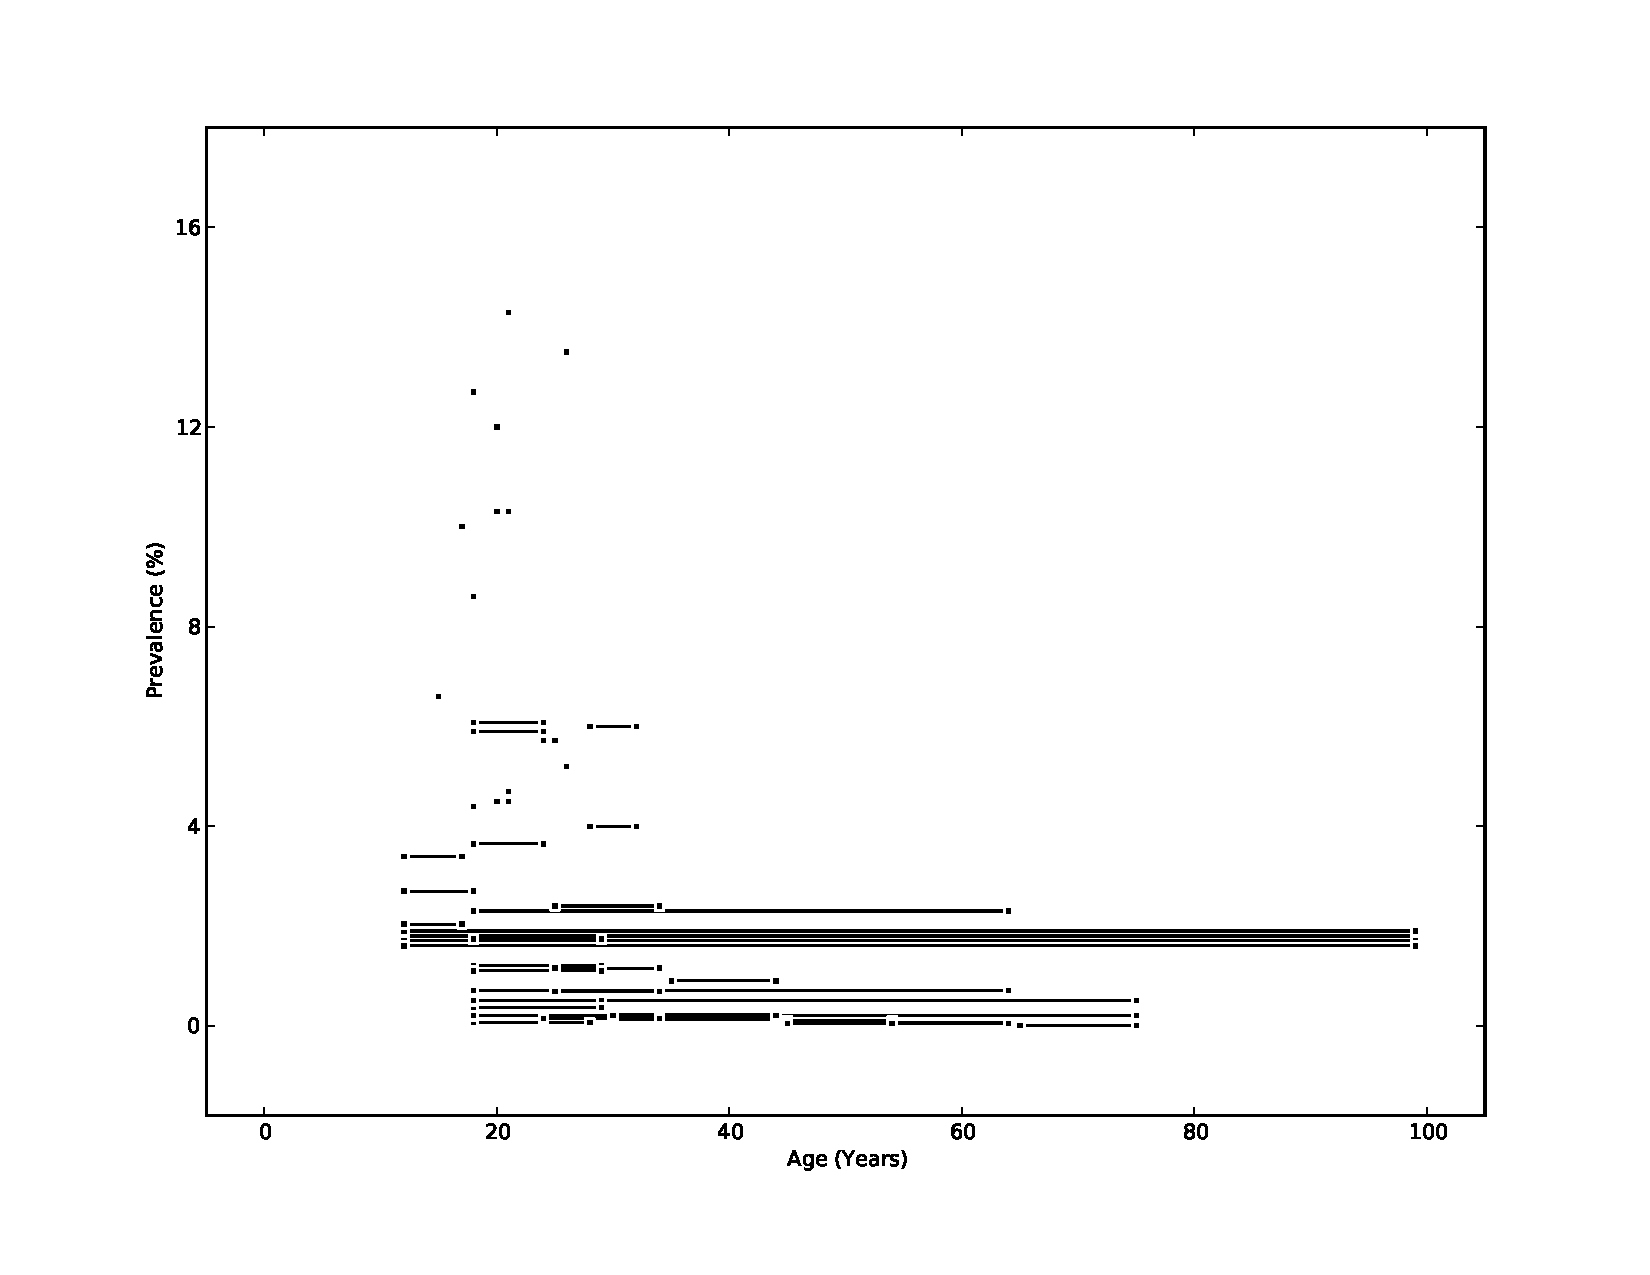
\includegraphics[width=\textwidth]{cannabis_dependence-data.pdf}
            \caption{Global data for cannabis dependence.}
            \label{fig:app-cannabis_data}
        \end{center}
    \end{figure}

As discussed in Chapter \ref{ch:theory-age_patten_model}, age-specific hazards are modeled with spline models.  A spline model is any piecewise polynomial function.  Knots partition the age range into intervals.  With ample data and clear age patterns, models will not be very sensitive to choice of knots.  However, when working with sparse and noisy data, the number and location of knots are important decisions as they can influence the model results substantially.  When this is the case, the number of knots and locations should be chosen a priori using expert knowledge concerning the disease being modeled.

The model for cannabis dependence has knots at the ages of 0, 13, 17, 22, 30, 35, 40, 45, 50, 60, and 100.  The less knot model limits knots to ages 0, 13, 25, 65, and 100.   During the critical period of 13-50 years, the more knot model has knots every three years (0, 13, 16, 19, �, 43, 46, 49) with additional knots at 55, 60, 80 and 100.  The most knot model has knots every two years during the ages of 13-66 (knots at ages 0, 13, 15, 17, �, 61, 63, 65, and 100). As seen in figure \ref{fig:app-cannabis_knots}, choosing too few or too many knots can influence the model substantially.

    \begin{figure}[h]
        \begin{center}
            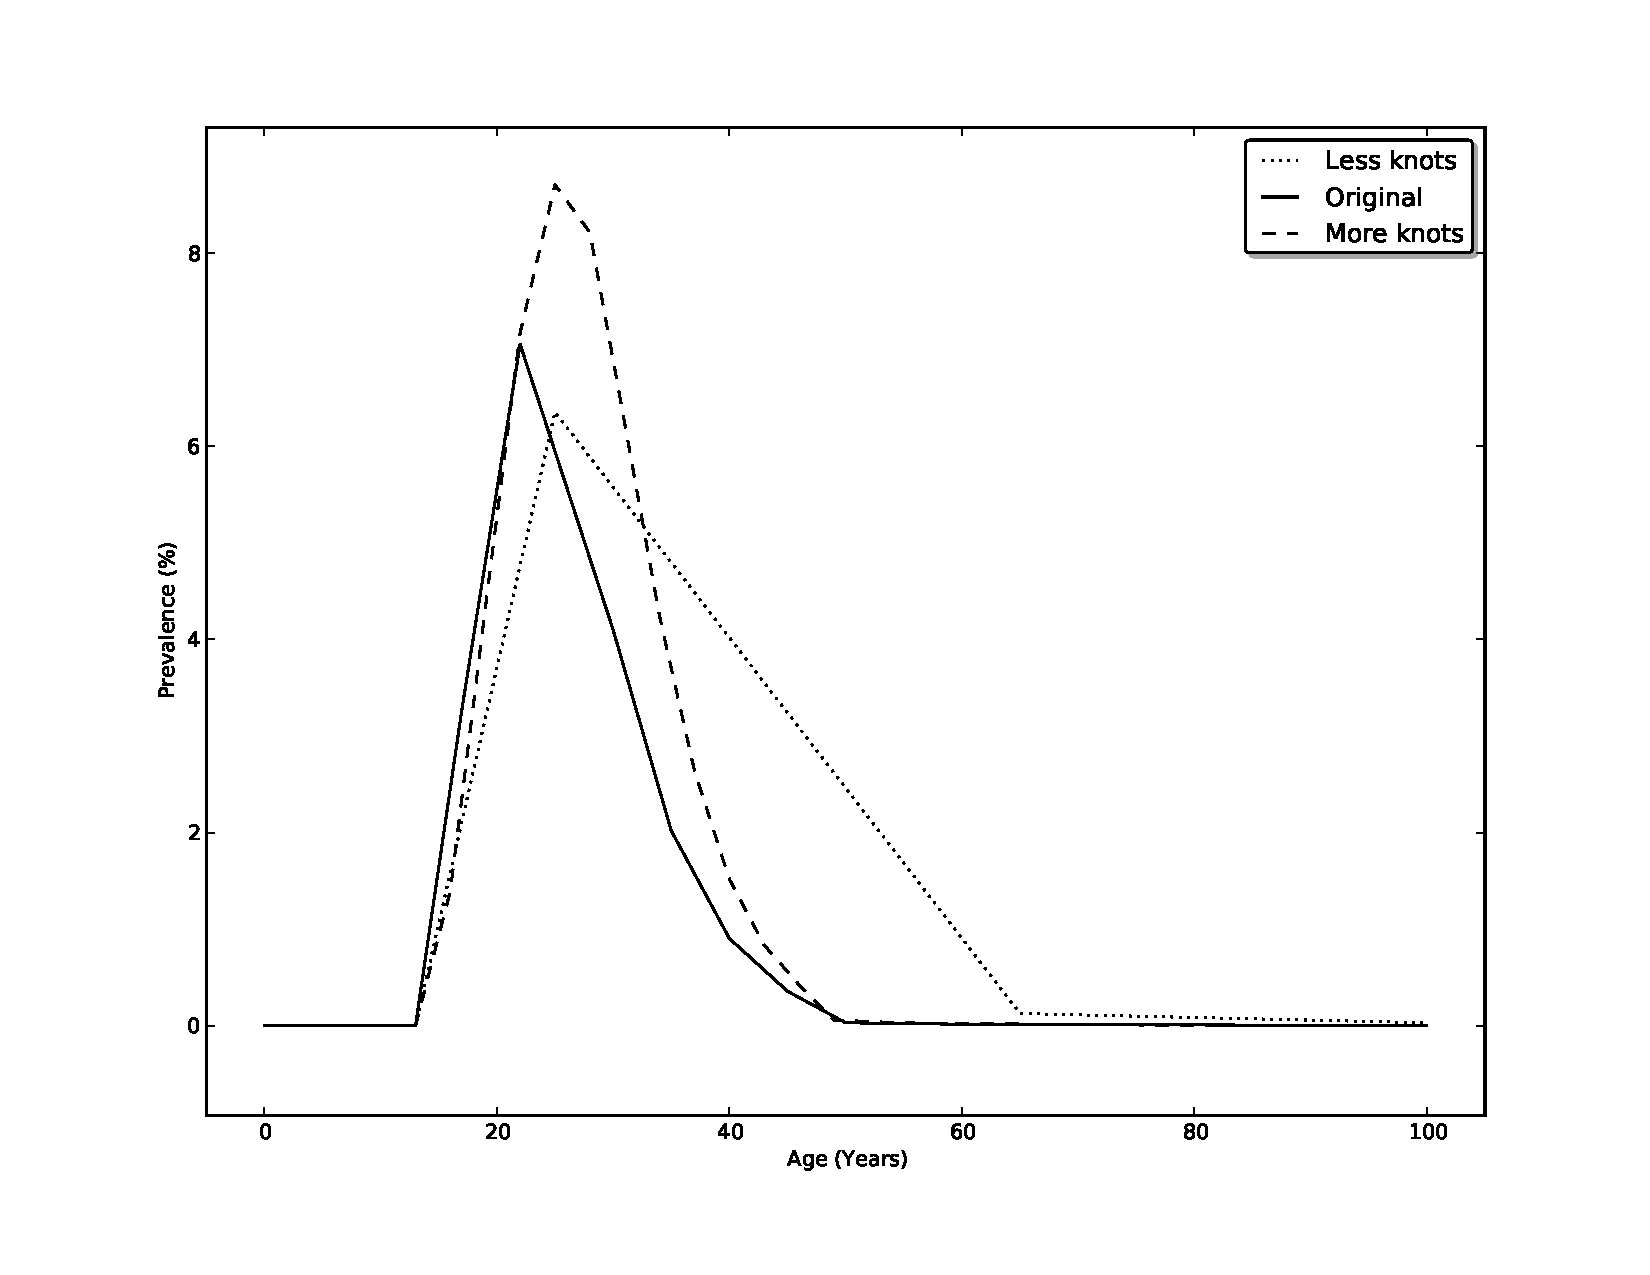
\includegraphics[width=\textwidth]{applications/cannabis_dependence-knots.pdf}
            \caption{Penalized splines with a smoothing parameter make knot selection less influential by penalizing use of unnecessary knots for data.  However, overcompression is not representative of the data.}
        \label{fig:app-cannabis_knots}
        \end{center}
    \end{figure} 